%!TEX root = ../cursus_fys6.tex

\chapter{De gravitatiekracht}

%Inleiding

%- Middeleeuws wereldbeeld
%
%- Aristoteles
%
%- Ptolemaeus
%
%- Het aantal engelen op een speldenkop + voetnoot
%
%- generalisatie, verhaaltje van appel, maar hoe zit het dan met kleine massa's

%\begin{figure}[h]
%\centering
%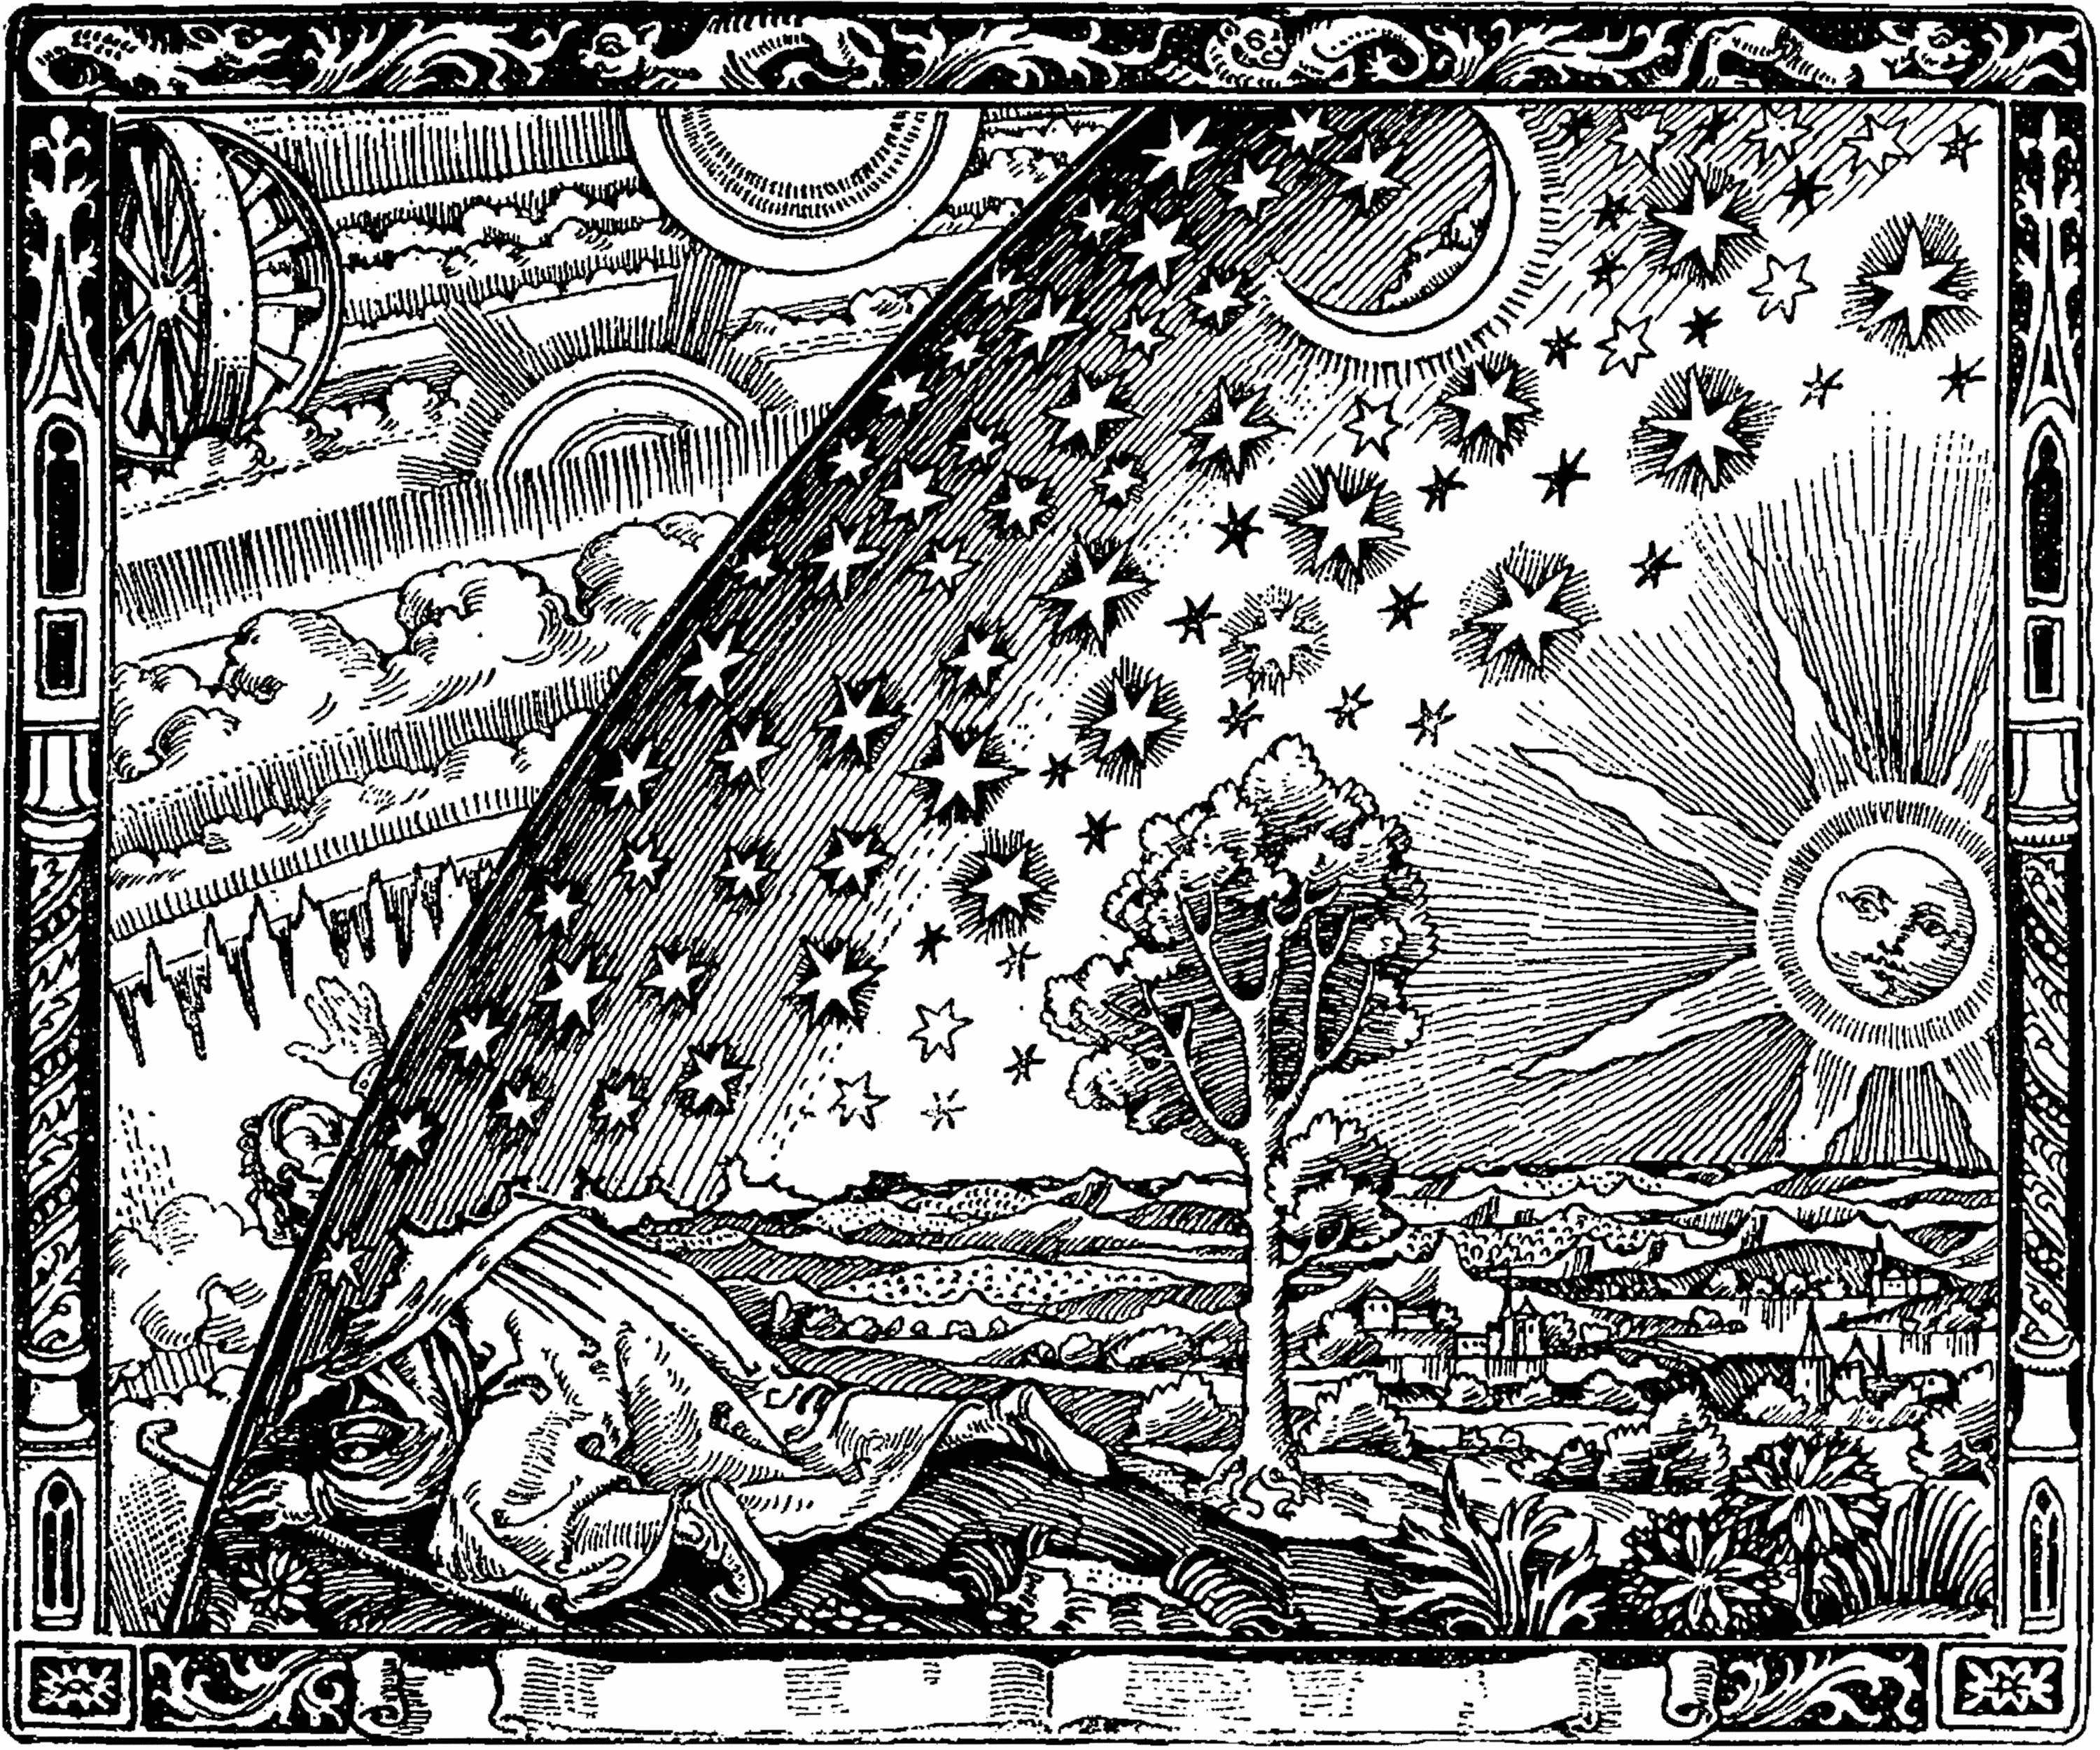
\includegraphics[width=0.9\textwidth]{flammarion}
%\caption{\textit{Flammarion gravure}. 1888.}
%\end{figure}

%\begin{figure}[h]
%\centering
%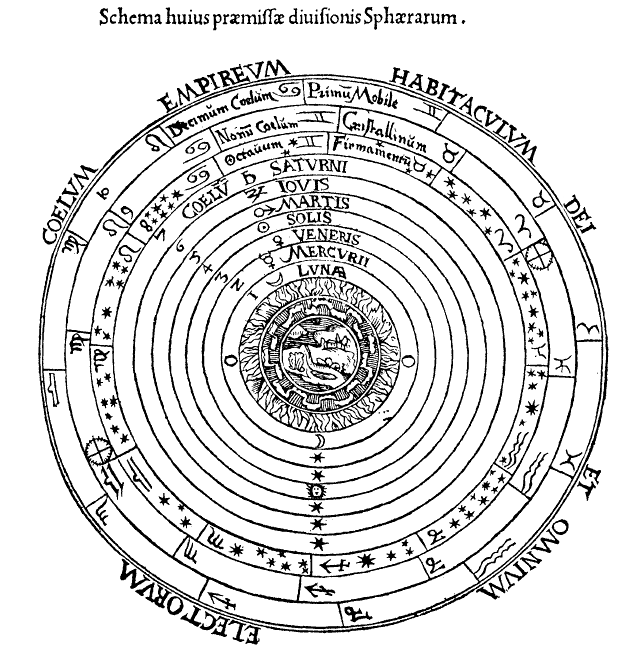
\includegraphics[width=0.9\textwidth]{Ptolemaicsystem-small}
%\caption{\textit{Schema huius praemissae divisionis sphaerarum.}}
%\end{figure}

%\newpage

\section{De wetten van Kepler}

Johannes Kepler (1571 - 1630) destilleerde uit de enorme hoeveelheid meetgegevens van planeetposities die Tycho Brahe (1546 - 1601) verzamelde, zijn drie wetten. Ze luiden: een planeet beweegt in een elliptische baan met de zon in een van de brandpunten, de voerstraal snijdt in gelijke tijdsintervallen gelijke oppervlakten (perken) uit (perkenwet) en de verhouding van het kwadraat van de periode tot de derde macht van de halve lange as van de ellipsbaan is voor alle planeten gelijk.

\section{De universele gravitatiekracht}

%- redenering maan

%- verklaring wetten Kepler

Isaac Newton (1642 - 1727) kon aantonen dat wanneer hij aannam dat planeten door de zon werden aangetrokken door een kracht die omgekeerd evenredig is met het kwadraat van de afstand, de drie wetten van Kepler hieruit af te leiden zijn. Daar waar de wetten van Kepler slechts inductief uit empirische gegevens zijn afgeleid, zijn ze bij Newton een gevolg van zijn bewegingsleer: de gravitatiekracht als oorzaak van beweging en zijn tweede wet als bewegingsvergelijking. Nu zijn de wetten een deductief gevolg uit een theoretisch model.

Een ander argument dat Newton gebruikte om zijn voorstel voor de formule van de universele gravitatiekracht te corroboreren\footnote{Een moeilijk woord dat `met argumenten staven' betekent.}, was een redenering over de versnelling van de maan.\footnote{Zijn berekeningen borg hij op omdat ze niet strookte met de realiteit. Enkele jaren later bleek echter dat de door astronomen gebruikte afstand tot de maan fout was. Een nieuwe waarde toonde aan dat Newton een correcte redenering had gebruikt.} Ze gaat als volgt. De maan maakt een nagenoeg cirkelvormige beweging. Haar versnelling is dus te berekenen met de formule voor de versnelling van een ECB. We hebben dan de omlooptijd en de afstand tot de maan nodig. De straal van de cirkelbeweging van de maan is ongeveer 60 keer de straal van de aarde.
\begin{eqnarray*}
	a&=&r\omega^2=r\left(\frac{2\pi}{T}\right)^2\\
	&=&6370\cdot10^3\rm\,m\cdot60\cdot\left(\frac{2\pi}{27,3\cdot24\cdot60\cdot60\rm\,s}\right)^2=0,0027\rm\,m/s^2
\end{eqnarray*}
Dit getal komt overeen met een omgekeerd kwadratische afhankelijkheid van de straal. Nemen we namelijk de valversnelling op aarde, $9,81\rm\,m/s^2$ en delen we deze door $60^2$ (de maan bevindt zich immers 60 keer zo ver), dan krijgen we hetzelfde getal.
\begin{eqnarray*}
	a=\frac{9,81\rm\,m/s^2}{60^2}=0,0027\rm\,m/s^2
\end{eqnarray*}
Hiermee had Newton een argument om aan te nemen dat de gravitatiekracht omgekeerd evenredig moet zijn met het kwadraat van de onderlinge afstand tussen de massa's.

De \textit{universele of algemene gravitatiekracht}, \'e\'en van de vier fundamentele natuurkrachten, wordt als volgt geformuleerd:
\begin{center}
\framebox{
\begin{minipage}[t]{\textwidth}
Twee puntmassa's $m$ en $m'$, die zich op een afstand $r$ van elkaar
bevinden, trekken elkaar aan met een kracht die gericht is volgens
de verbindingslijn van de twee massa's en waarvan de grootte recht
evenredig is met het product van de twee massa's en omgekeerd
evenredig met het kwadraat van de afstand tussen beide:
\begin{eqnarray}\label{universele gravitatiekracht}
F&=&G\frac{mm'}{r^2}
\end{eqnarray}
De evenredigheidsco\"effici\"ent $G$ wordt de
\textit{gravitatieconstante} genoemd.
\begin{eqnarray}\label{gravitatieconstante}\nonumber
G&=&6,67\cdot10^{-11}\rm\,\frac{Nm^2}{kg^2}
\end{eqnarray}
\end{minipage}}
\end{center}

Newton bepaalde de constante $G$ niet zelf. Dat werd na zijn dood door Cavendish (1731 - 1810) gedaan.

\newpage

\section{Satellietbanen}

Hoe komt het dat de maan door de aarde wordt aangetrokken en er toch niet naartoe valt? Dat komt omdat de neiging van de maan om door de traagheid weg te vliegen volgens de richting waarin hij beweegt, de valbeweging naar de aarde toe compenseert. De gravitatiekracht zorgt voor de middelpuntzoekende kracht van de nagenoeg cirkelvormige beweging die de maan maakt rond de aarde.\footnote{Maar welke kracht duwt de maan dan voort om zijn snelheid te onderhouden? Geen kracht! Herinner je dat de wet van de traagheid zegt dat je geen kracht nodig hebt om een eenmaal verworven snelheid aan te houden. Er is ook geen directe maar een indirecte relatie tussen kracht en snelheid. De tweede wet van Newton relateert kracht aan \textit{versnelling}, niet aan snelheid! Omdat er in de ruimte geen wrijving is, is er niemand om de maan tegen te houden en blijft hij voortgaan.}

Net zoals de maan worden ook kunstsatellieten door de gravitatiekracht in een baan rond de aarde gehouden. Denk maar aan GPS-satellieten en het internationaal ruimtestation. Op de website van de NASA\footnote{\href{http://science.nasa.gov/iSat/}{iSat: Interactive Satellite Viewer (science.nasa.gov/iSat/)}} kan je real-time gegevens van verschillende satellieten terugvinden.

\subsection{Parkeerbaan}

Met een satelliet is het net zoals met de maan. Willen we ervoor zorgen dat de satelliet steeds in eenzelfde baan ronde de aarde blijft cirkelen, dan moet hij een welbepaalde snelheid meekrijgen. Voor een cirkelvormige baan met de aarde als middelpunt fungeert de gravitatiekracht als middelpuntzoekende kracht. De versnelling is dan die van een ECB, wat we kunnen gebruiken om de juiste snelheid af te leiden:
\begin{eqnarray*}
F&=&ma\\
G\frac{m_am}{r^2}&=&m\frac{v^2}{r}\\
v&=&\sqrt{\frac{Gm_a}{r}}
\end{eqnarray*}
Hierin is $m$ de massa van de satelliet, $m_a$ de massa van de aarde en $r$ de straal van de cirkelbeweging die de satelliet maakt. De massa van de satelliet speelt duidelijk geen rol. 

Passen we deze formule toe op het internationaal ruimtestation, dat ongeveer op een hoogte van $412\rm\,km$ vliegt, dan krijgen we, met een gemiddelde aardstraal van $6370\rm\,km$, volgende schatting voor de snelheid:
\begin{eqnarray*}
	v=\sqrt{\frac{6,67\cdot10^{-11}\rm\,\frac{Nm^2}{kg^2}\cdot5,9721986\cdot10^{24}\rm\,kg}{6370\cdot10^3\rm\,m+412\cdot10^3\rm\,m}}=7,66\rm\,km/s
\end{eqnarray*}
Dit ligt erg dicht bij de eigenlijke snelheid -- en dat voor zo'n `simpele' berekening. De mechanica van Newton is duidelijk heel krachtig!

\subsection{Geostationaire baan}

Er is \'e\'en satellietbaan die een speciale eigenschap heeft: de snelheid van de satelliet en de afstand tot de aarde zijn zodanig dat de hoeksnelheid van de satelliet gelijk is aan die van de aarde. De baan ligt bovendien in het equatoriaal vlak zodat voor een waarnemer op de evenaar de satelliet steeds zichtbaar is in het zenit -- loodrecht boven de waarnemer. Vandaar dat over een geostationaire baan wordt gesproken.

Als we eisen dat de hoeksnelheid van de satelliet gelijk is aan die van de aarde (de periode moet bijgevolg 24 uur zijn) en dat de baan in het evenaarsvlak ligt, kunnen we de straal van de baan afleiden:
\begin{eqnarray*}
F&=&ma\\
&\Downarrow&\\
G\frac{m_am}{r^2}&=&mr\omega^2\\
r&=&\sqrt[3]{\frac{Gm_a}{\omega^2}}=\sqrt[3]{\frac{Gm_aT^2}{4\pi^2}}\\
&=&\sqrt[3]{\frac{6,67\cdot10^{-11}\rm\,\frac{Nm^2}{kg^2}\cdot5,9721986\cdot10^{24}\rm\,kg\cdot(24\cdot60\cdot60\rm\,s)^2}{4\pi^2}}\\
&=&42\,232\rm\,km
\end{eqnarray*}
Als we hier de straal van de aarde nog afhalen, vinden we dat de satellietbaan zich $42\,232\rm\,km-6\,370\rm\,km=35\,862\rm\,km$ boven het aardoppervlak bevindt. Dat is ongeveer een tiende van de afstand tot de maan.

\textit{Opmerking}: waarom kan er geen geostationaire baan boven Belgi\"e worden ge\"installeerd? Omdat alle parkeerbanen als middelpunt het middelpunt van de aarde moeten hebben. Het is immers de gravitatiekracht die voor de middelpuntzoekende kracht zorgt. Moest je een baan boven Belgi\"e willen maken, dan zou het middelpunt op de rotatieas ergens boven de noordpool liggen. Vanuit dat middelpunt wordt echter geen kracht uitgeoefend.


\section{Gewicht}

%- insteek via gewichtloos zijn in de ruimte

%- gewicht is hoeveel het weegt, de impact. Weegschaal?... Afwegen? Belang van iets, gewichtig? > voetnoot

%\begin{center}
\framebox{
\begin{minipage}[t]{\textwidth}
Het gewicht van een lichaam is de grootte van de kracht die door het lichaam op haar steun wordt uitgeoefend.
\end{minipage}}
%\end{center}

Let op het feit dat het om de \textit{grootte} van een kracht gaat en dat gewicht dus wordt uitgedrukt in newton. In de omgangstaal zijn we hierin niet correct. Men zegt zoveel kilogram te wegen terwijl kilogram de eenheid van massa is.

%- voorbeeld met een lift.


\section{De zwaartekracht}
De zwaartekracht is een bijzonder geval van de universele gravitatiekracht: de gravitatiekracht door de aarde op een massa uitgeoefend noemen we ook de zwaartekracht.

\subsection{De valversnelling}

Proefondervindelijk zien we dat op de aarde alle lichamen met
dezelfde valversnelling $g$ naar de aarde toe vallen. De tweede wet
van Newton zegt dan dat de zwaartekracht die deze versnelling moet
veroorzaken gelijk moet zijn aan de massa van het lichaam
vermenigvuldigd met deze versnelling:
%\begin{eqnarray*}
%F_z&=&mg
%\end{eqnarray*}
%Deze vergelijking geeft dus aan \textit{hoe groot} de kracht moet
%zijn. Het \textit{is} echter de universele gravitatiekracht door de
%aarde op de massa uitgeoefend. Er moet dus gelden:
\begin{eqnarray}
F&=&ma\nonumber\\
&\Downarrow&\nonumber\\
G\frac{m_Am}{r^2}&=&mg\nonumber\\
&\Updownarrow&\nonumber\\
g&=&G\frac{m_A}{r^2}
\end{eqnarray}
De valversnelling $g$ is inderdaad onafhankelijk van de massa van
het be\-schouw\-de lichaam.

De zwaartekracht op een grotere massa is wel groter, maar doordat
een grotere massa een grotere traagheid heeft, is het moeilijker haar
bewegingstoestand te veranderen. Deze twee eigenschappen heffen
elkaar dus op zodat alle massa's met een zelfde valversnelling vallen.

%\subsection{$g$ is geen constante}

%- factoren die $g$ be\"invloeden

%- welke benadering hebben we eigenlijk gemaakt?

%\clearpage
%\newpage
